\chapter{Applicability to Amputee Data}
\label{chp:amputee-data}

The collection of labelled training data is arduous; this problem becomes more acute when the subject has restricted movement, such as an amputee. Therefore, any system that can reduce these individuals' data requirements is of benefit. In Chapter \ref{chp:personalisation}, methods for personalisation of a machine learning model using additional data from other subjects were demonstrated to improve the model's performance and reduce the data requirements for that model. Within this Chapter, these methods will be implemented for an amputee to investigate if they apply to someone with an impaired gait.

The contributions of this Chapter are:
\begin{itemize}
    \item Collection of amputee gait data that is directly comparable to non-amputee data
    \item Comparison of shank \acrshort{marg} data between non-amputee, intact limb and prosthetic
    \item Demonstration of performance differences of \acrshort{lmr} network of intact and prosthetic side
    \item Demonstration of transfer learning from non-amputee data to an amputee for \acrshort{marg} gait data
\end{itemize}

First Section \ref{sec:amputee-methods} explains the methods used, and presents the collected amputee data. Following this in Sections \ref{sec:amputee-baseline}, \ref{sec:amputee-supplementation} and \ref{sec:amputee-transfer} present the results of a baseline model performance and performance of two personalisation methods, respectively. Finally, the discussion and conclusion are given in Section \ref{sec:amputee-discussion}.

From the literature the following gaps were identified:
\begin{itemize}
    \item No work has attempted to use transfer learning to personalise a non-amputee \acrshort{lmr} model for an amputee
    \item No papers have investigated the difference in classification performance between amputated and in-tact limb
\end{itemize}

The remainder of this Chapter will focus on investigating these gaps.

%-----------------------------------------------------------------
\section{Methods and Materials}
\label{sec:amputee-methods}
% Recap methods and what has changed
The methods used in this Chapter will mirror those used in previous chapters. Additional data for an amputee was collected. This was used to generate a new set of baselines to compare against and implement the previously developed personalisation methods. Complete tables of results for all experiments can be found in Appendix \ref{chp:tables-of-results} Section \ref{sec:app-a-amputee-transfer-learning}.

Data was collected from a single left trans-tibial amputee wearing a Blatchford Echelon VT prosthetic limb. Blatchford Product Limited collected the data. The data was collected in the same manner as previously described; however, a clinician at the centre held the smartphone to annotate activities to reduce the fall risk for the amputee. Data was collected walking around Blatchford's site in Basingstoke, both inside and outside. Table \ref{tab:summary-of-episode-amputee-data} summarises the data collected, including the number of data samples and the number of episodes for each activity.

\begin{table}[hbt]
    \centering
    \caption{Summary of amputee gait data collected}
    \label{tab:summary-of-episode-amputee-data}
    \begin{tabularx}{\textwidth}{c *{6}{Y}}
        \noalign{\hrule height 1.5pt}
        \textbf{Activity} & WALK  & \glsentryshort{ra} & \glsentryshort{rd} & \glsentryshort{sa} & \glsentryshort{sd} & STOP  \\
        \hline
        \textbf{Samples}  & 38114 & 6159               & 7194               & 2872               & 2450               & 11763 \\
        \textbf{Episodes} & 26    & 7                  & 7                  & 4                  & 4                  & 15    \\
        \noalign{\hrule height 1.5pt}                                                                                         \\
    \end{tabularx}
\end{table}

As significantly less data is available to test with, adjustments had to be made to the quantities used in each data set. The test data set was reduced from 5000 windows to 250 windows. The range of training windows tested was reduced to between 100 and 750. Additionally, to ensure that there were sufficient episodes for \acrshort{sa} and \acrshort{sd}, each of the stair episodes was split up into new episodes containing a maximum of 200 samples each. This increased the amount of available episodes for both stair activities.

Due to asymmetry, the left and right ankle data cannot be combined. This will be described further in the following section. All other quantities and hyper-parameters remained the same.

\subsection{Amputee Gait Data}
Gait asymmetry of amputees means that, unlike in the previous Chapter, the left and right ankle data cannot be combined to increase the dataset size. Instead, both sides will be evaluated independently to investigate the performance differences between the side. Figure \ref{fig:ch6_amputee_gyro_trends} shows the angular velocity of the shank in the sagittal plane for the intact and prosthetic limbs of a left amputated trans-tibial amputee. The left ankle has been transformed, so both ankles are presented in the same axes. For comparison, the ankle angular velocity of the non-amputee subject one is shown.

% How does it differ from non-amputee gait data
\begin{figure}[p]
    \begin{tabular}{lccc}
                                                                                                                                                 & \textbf{Non-Amputee}                                                                                                                  & \textbf{Amputee -- Prosthetic} & \textbf{Amputee -- Intact Limb} \vspace{0.2cm} \\

        \rotatebox{90}{\enspace\qquad \textbf{Walking}}                                                                                          &
        \begin{subfigure}[b]{0.275\textwidth}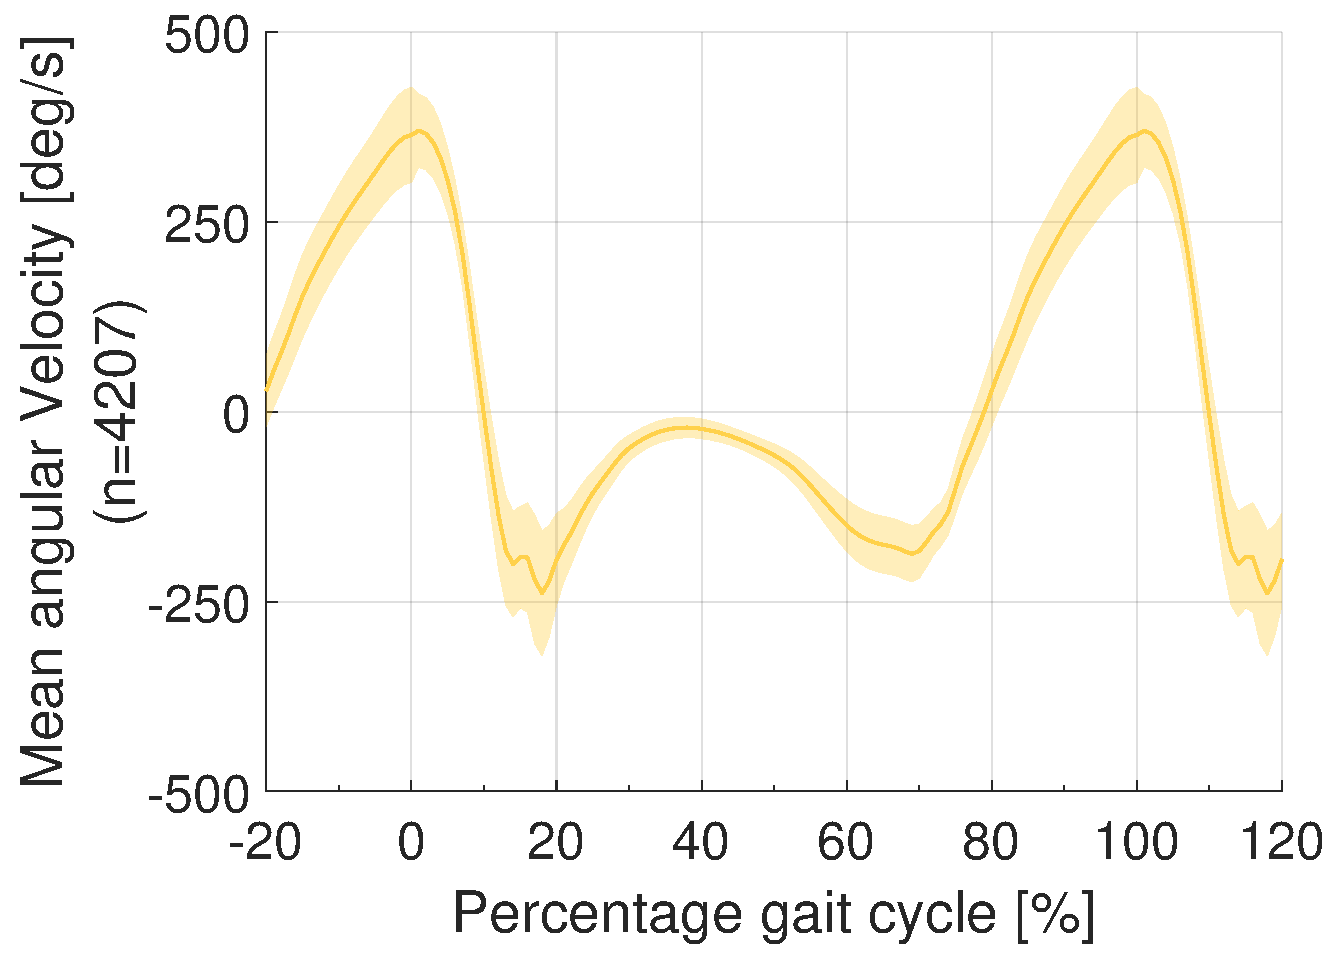
\includegraphics[width=\linewidth]{content/6-Amputee/Gait-Trends/ch6_subject_01_gait_trends_r_ankle_gyro_z_activity_walking.pdf}\end{subfigure}                                                                                                                & \begin{subfigure}[b]{0.275\textwidth}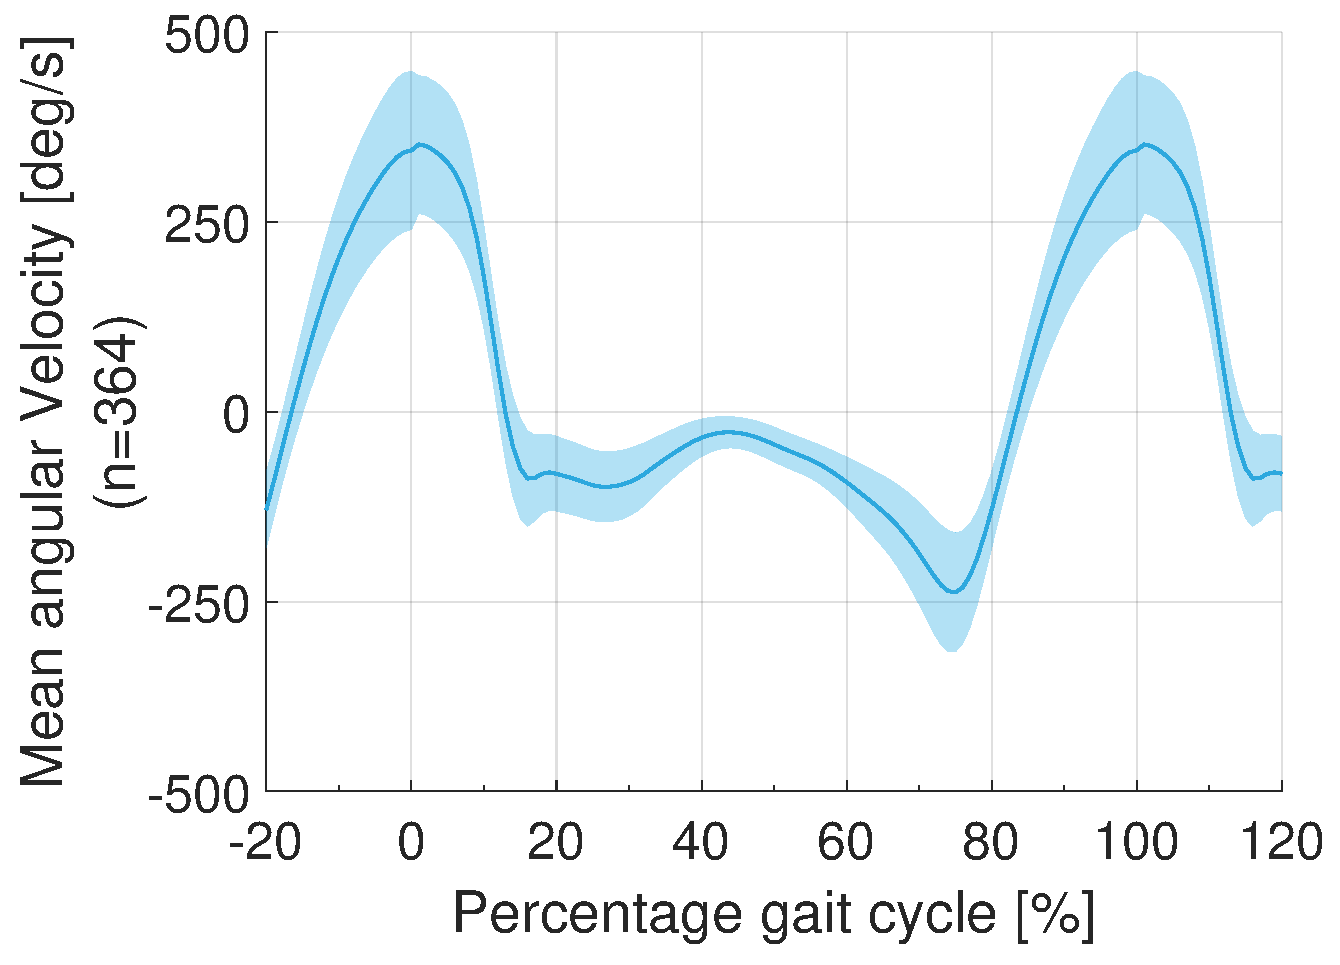
\includegraphics[width=\linewidth]{content/6-Amputee/Gait-Trends/ch6_amputee_gait_trends_l_ankle_gyro_z_activity_walking.pdf}\end{subfigure}                                                                                                             &
        \begin{subfigure}[b]{0.275\textwidth}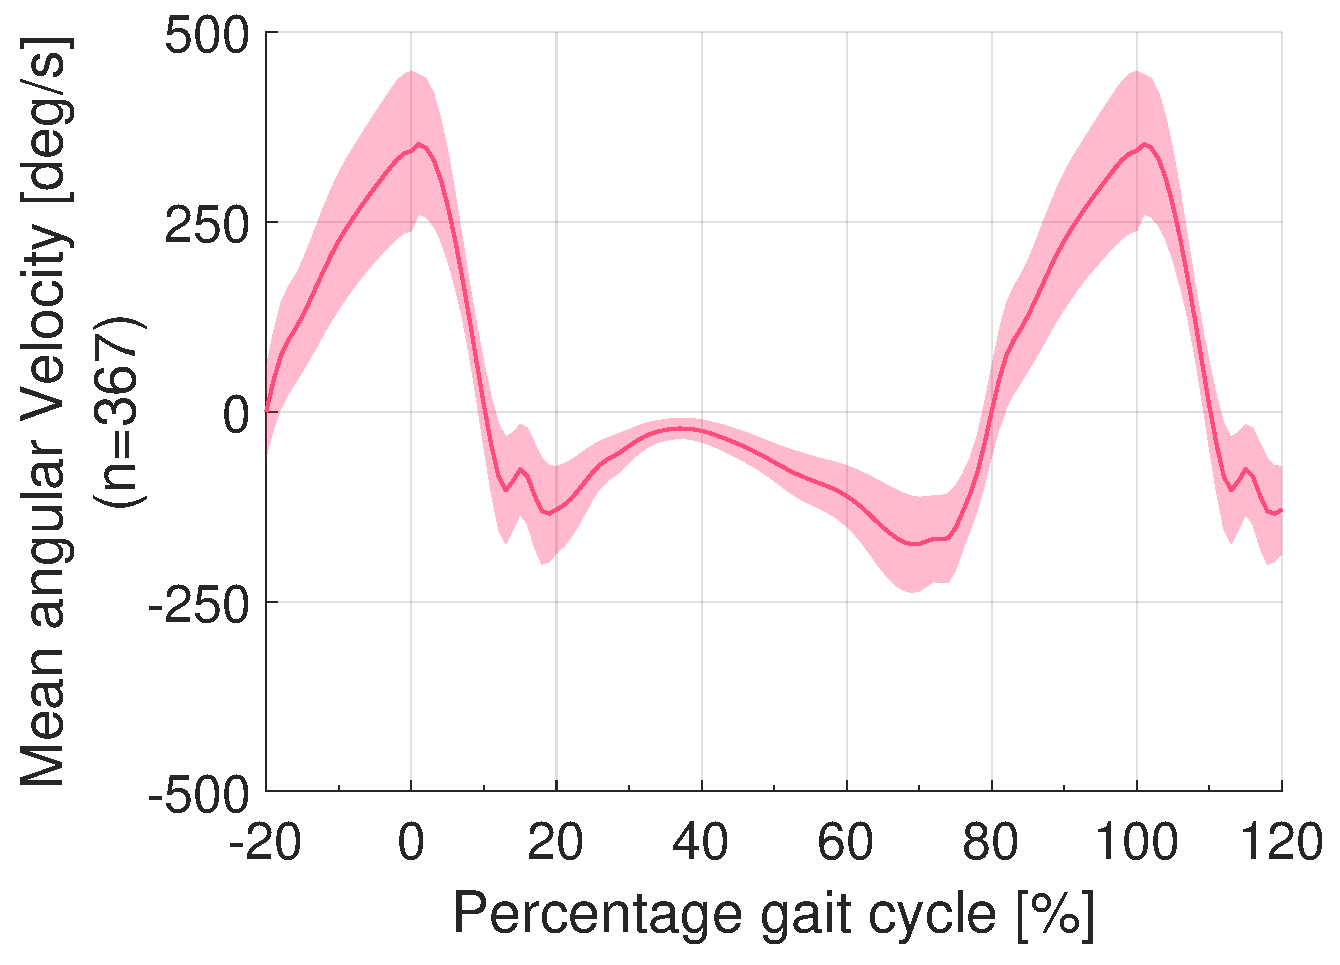
\includegraphics[width=\linewidth]{content/6-Amputee/Gait-Trends/ch6_amputee_gait_trends_r_ankle_gyro_z_activity_walking.pdf}\end{subfigure}                                                                                                                                                                                                                                                                                                                                          \\

        \rotatebox{90}{~\quad \textbf{Ramp Ascent}}                                                                                              &
        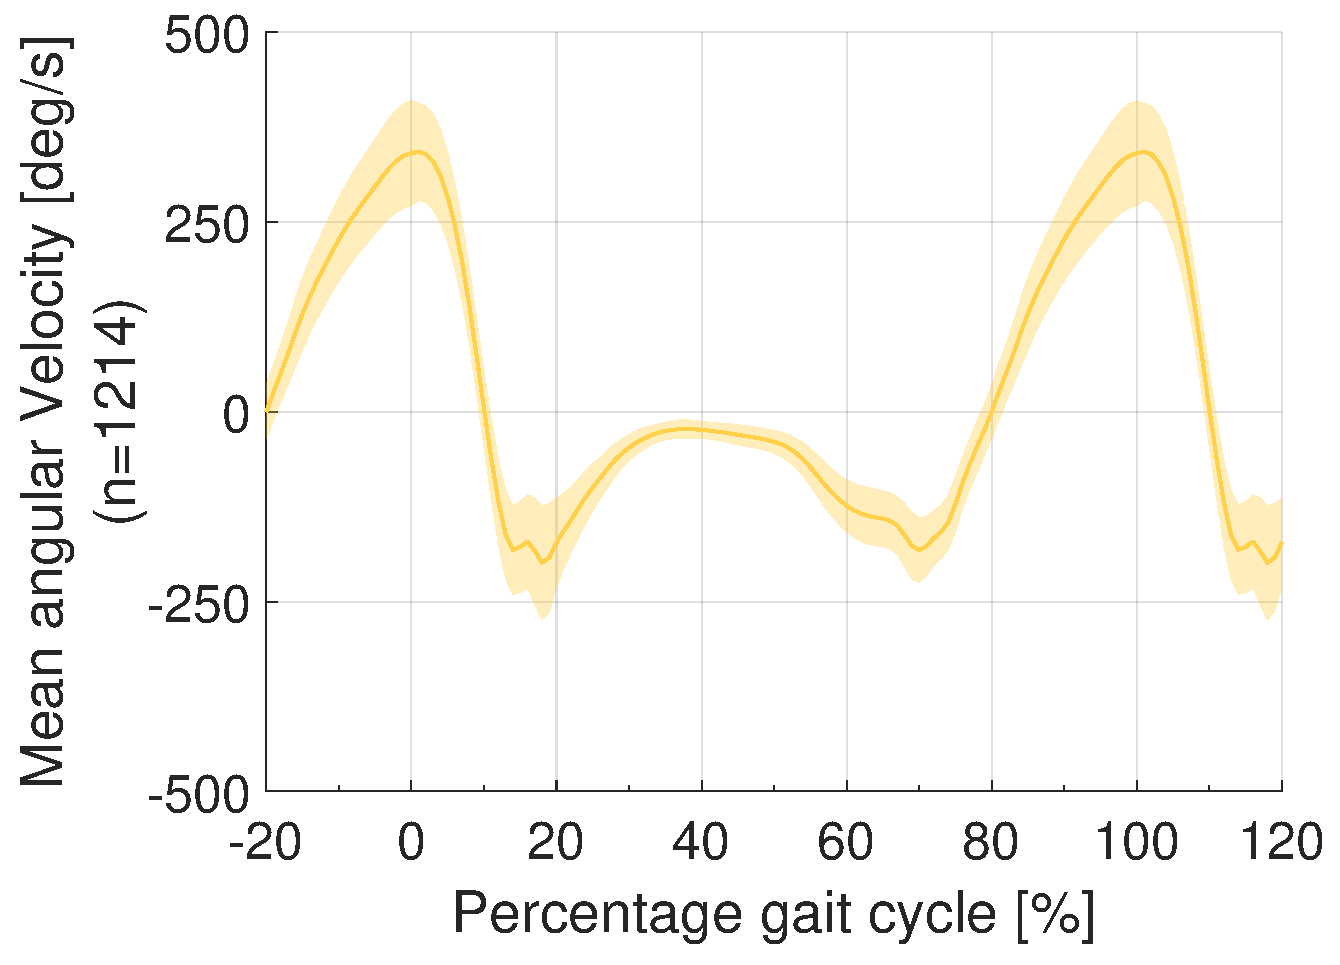
\includegraphics[width=0.275\linewidth]{content/6-Amputee/Gait-Trends/ch6_subject_01_gait_trends_r_ankle_gyro_z_activity_ramp_up.pdf}    & 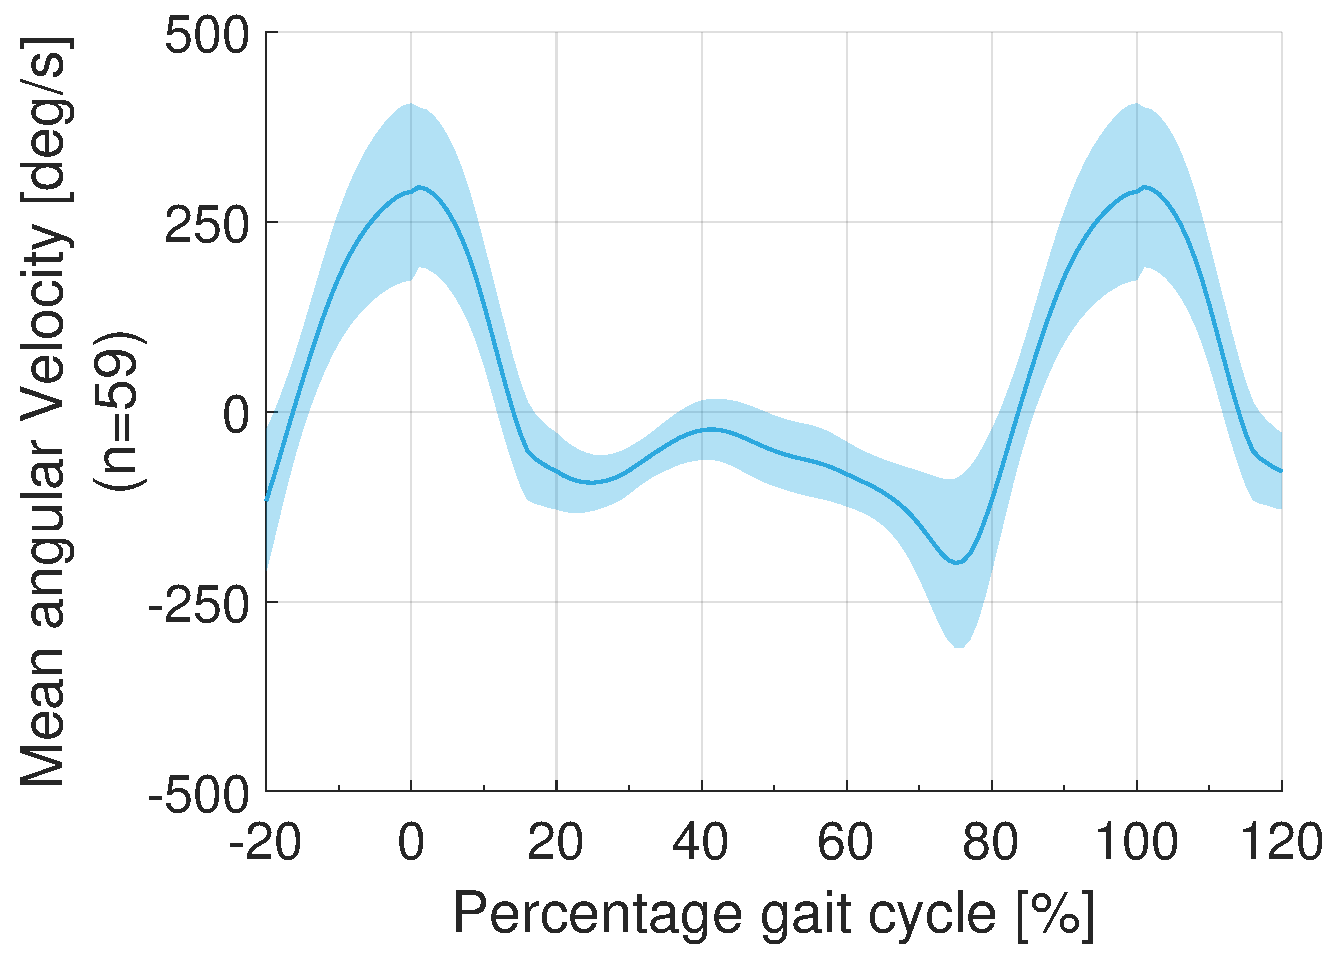
\includegraphics[width=0.275\linewidth]{content/6-Amputee/Gait-Trends/ch6_amputee_gait_trends_l_ankle_gyro_z_activity_ramp_up.pdf}    &
        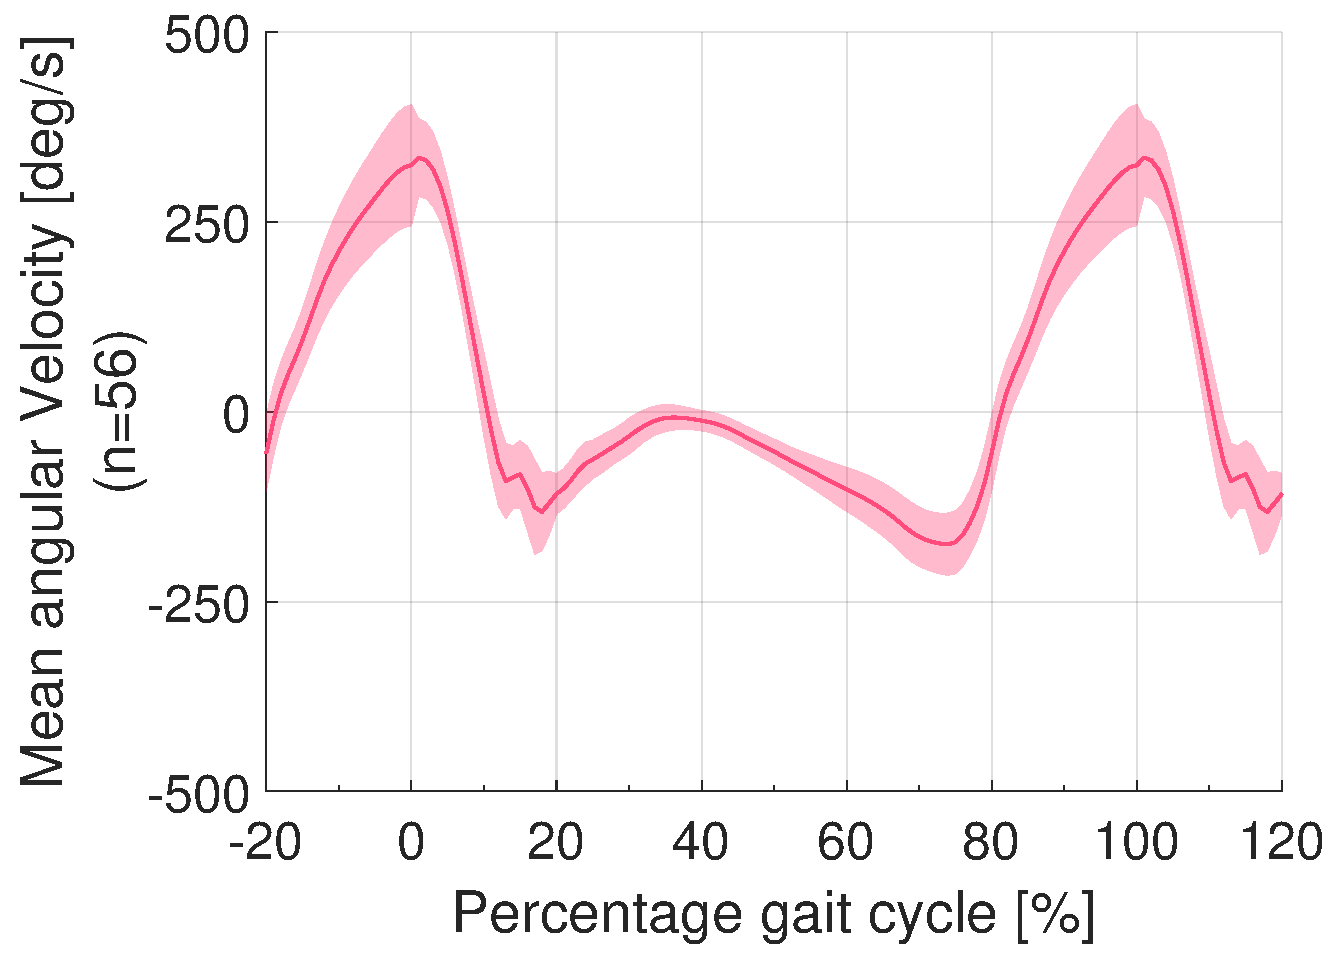
\includegraphics[width=0.275\linewidth]{content/6-Amputee/Gait-Trends/ch6_amputee_gait_trends_r_ankle_gyro_z_activity_ramp_up.pdf}                                                                                                                                                                                                                                 \\

        \rotatebox{90}{\quad \textbf{Ramp Descent}}                                                                                              &
        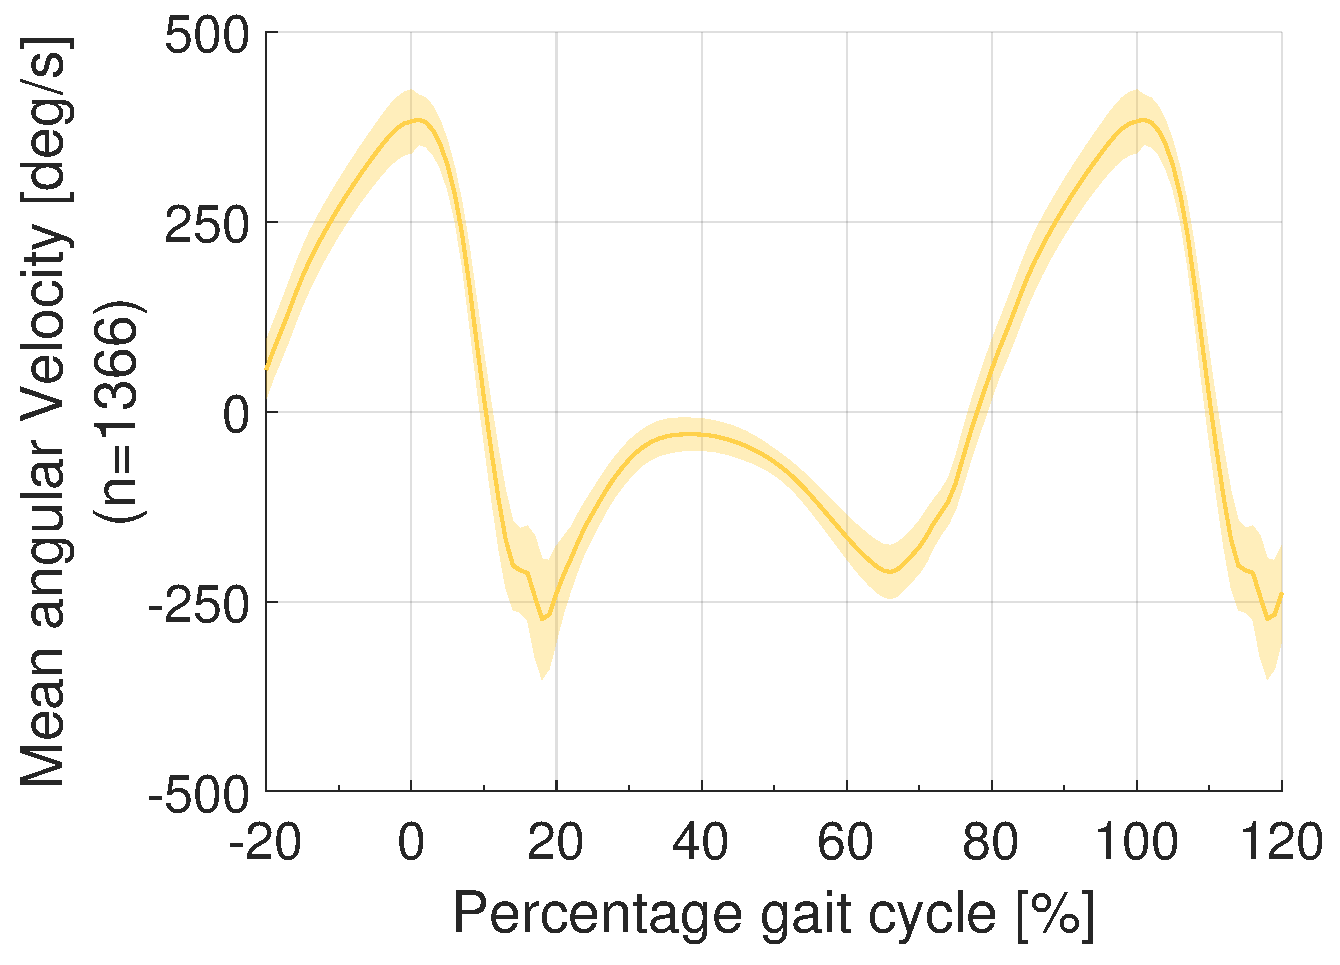
\includegraphics[width=0.275\linewidth]{content/6-Amputee/Gait-Trends/ch6_subject_01_gait_trends_r_ankle_gyro_z_activity_ramp_down.pdf}  & 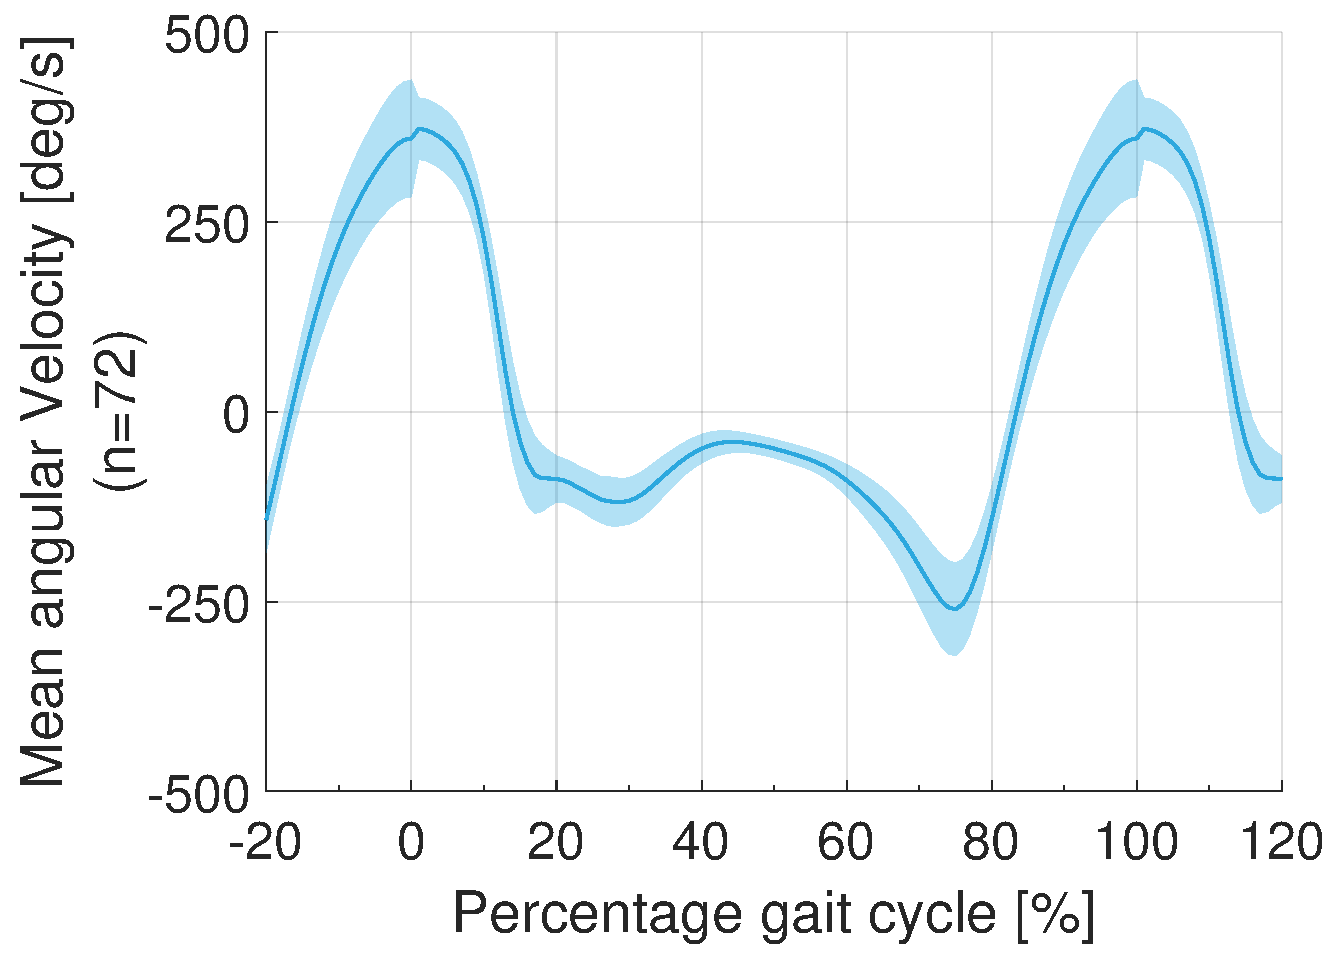
\includegraphics[width=0.275\linewidth]{content/6-Amputee/Gait-Trends/ch6_amputee_gait_trends_l_ankle_gyro_z_activity_ramp_down.pdf}  &
        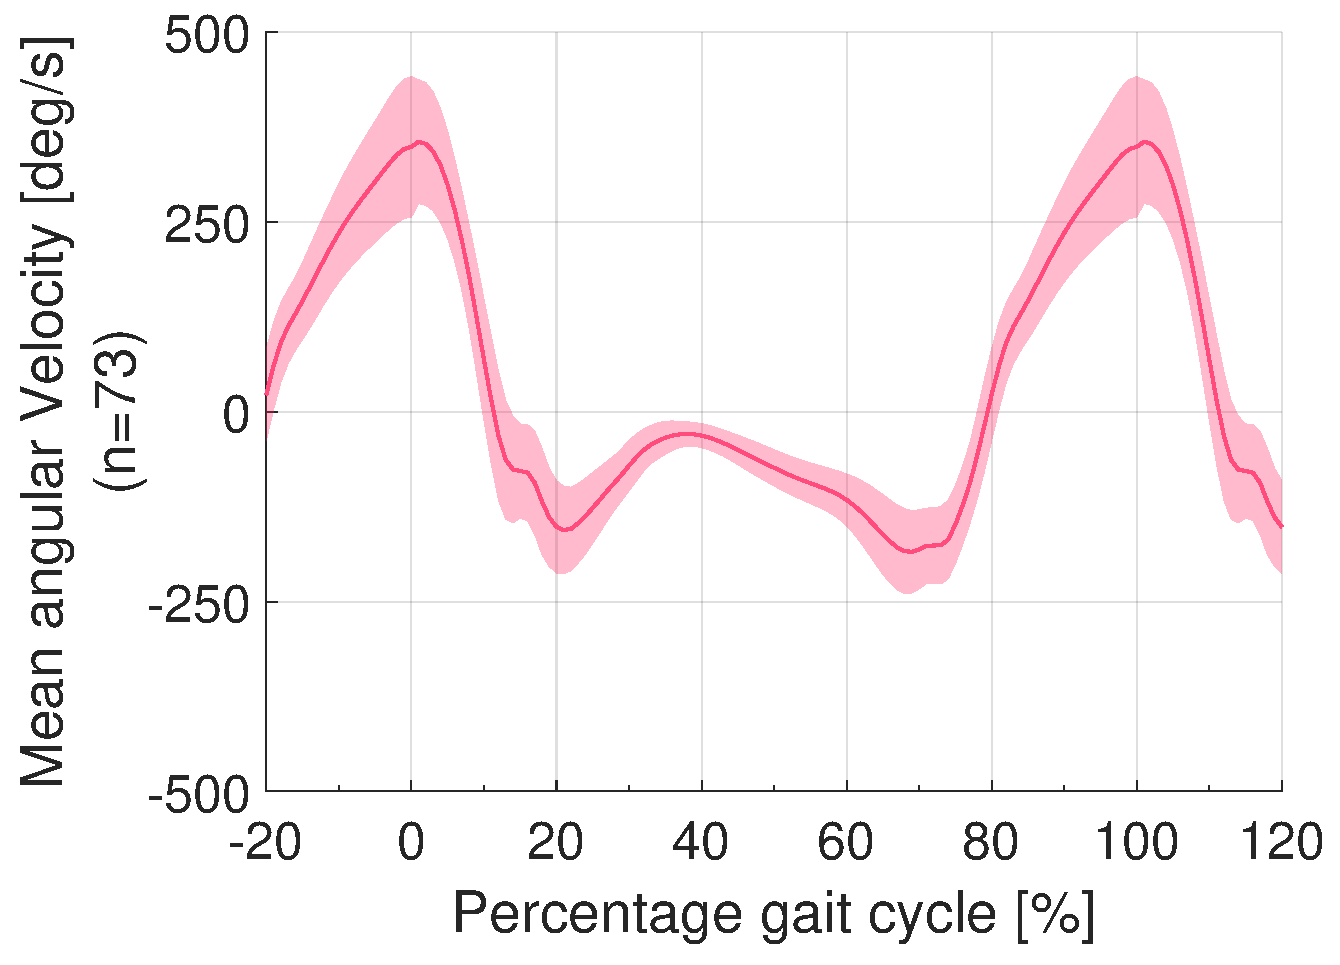
\includegraphics[width=0.275\linewidth]{content/6-Amputee/Gait-Trends/ch6_amputee_gait_trends_r_ankle_gyro_z_activity_ramp_down.pdf}                                                                                                                                                                                                                               \\

        \rotatebox{90}{~\quad \textbf{Stair Ascent}}                                                                                             &
        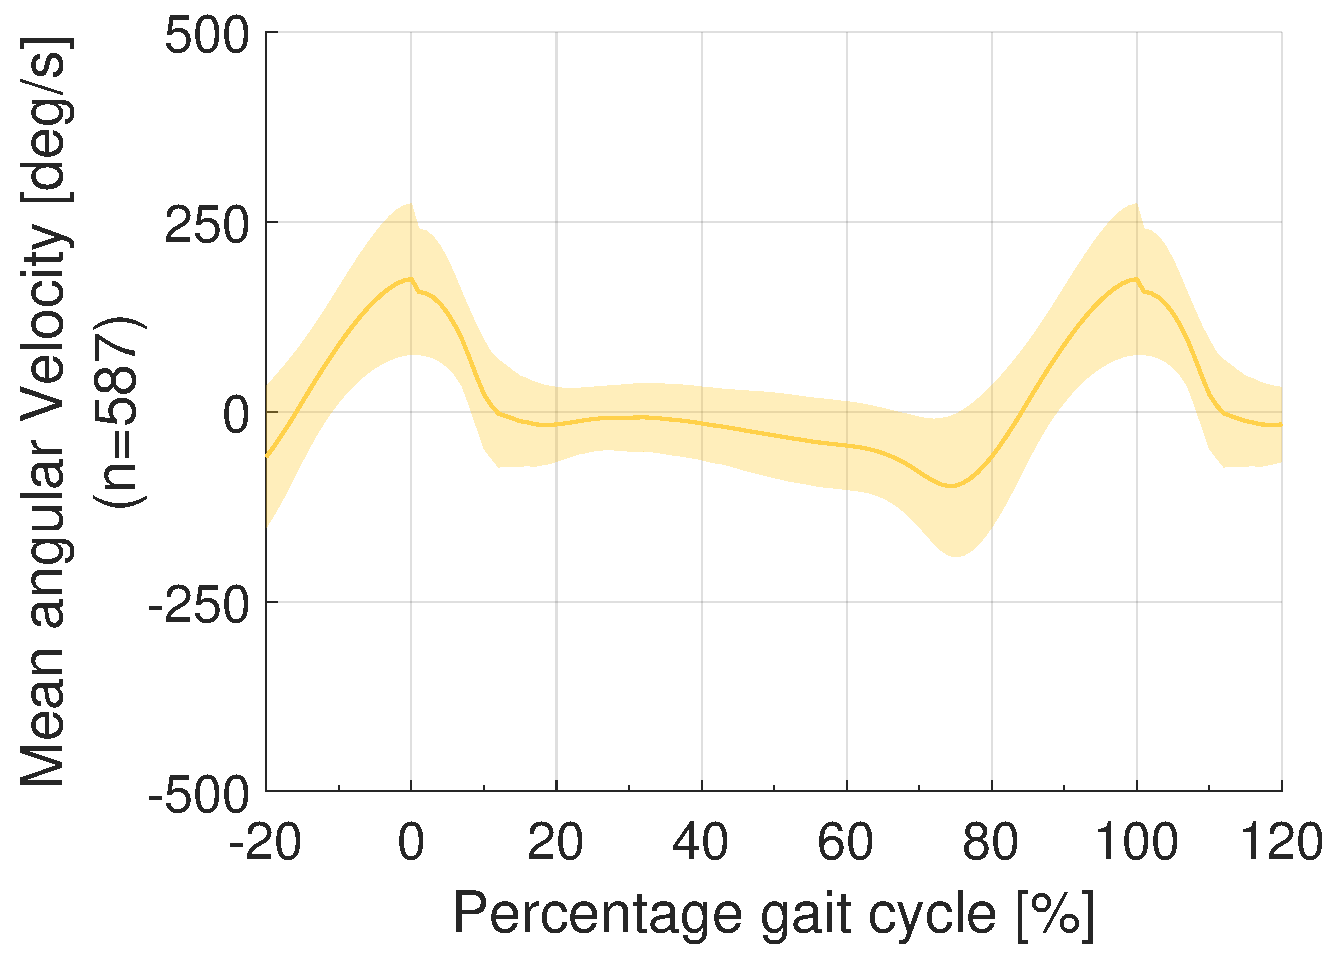
\includegraphics[width=0.275\linewidth]{content/6-Amputee/Gait-Trends/ch6_subject_01_gait_trends_r_ankle_gyro_z_activity_stair_up.pdf}   & 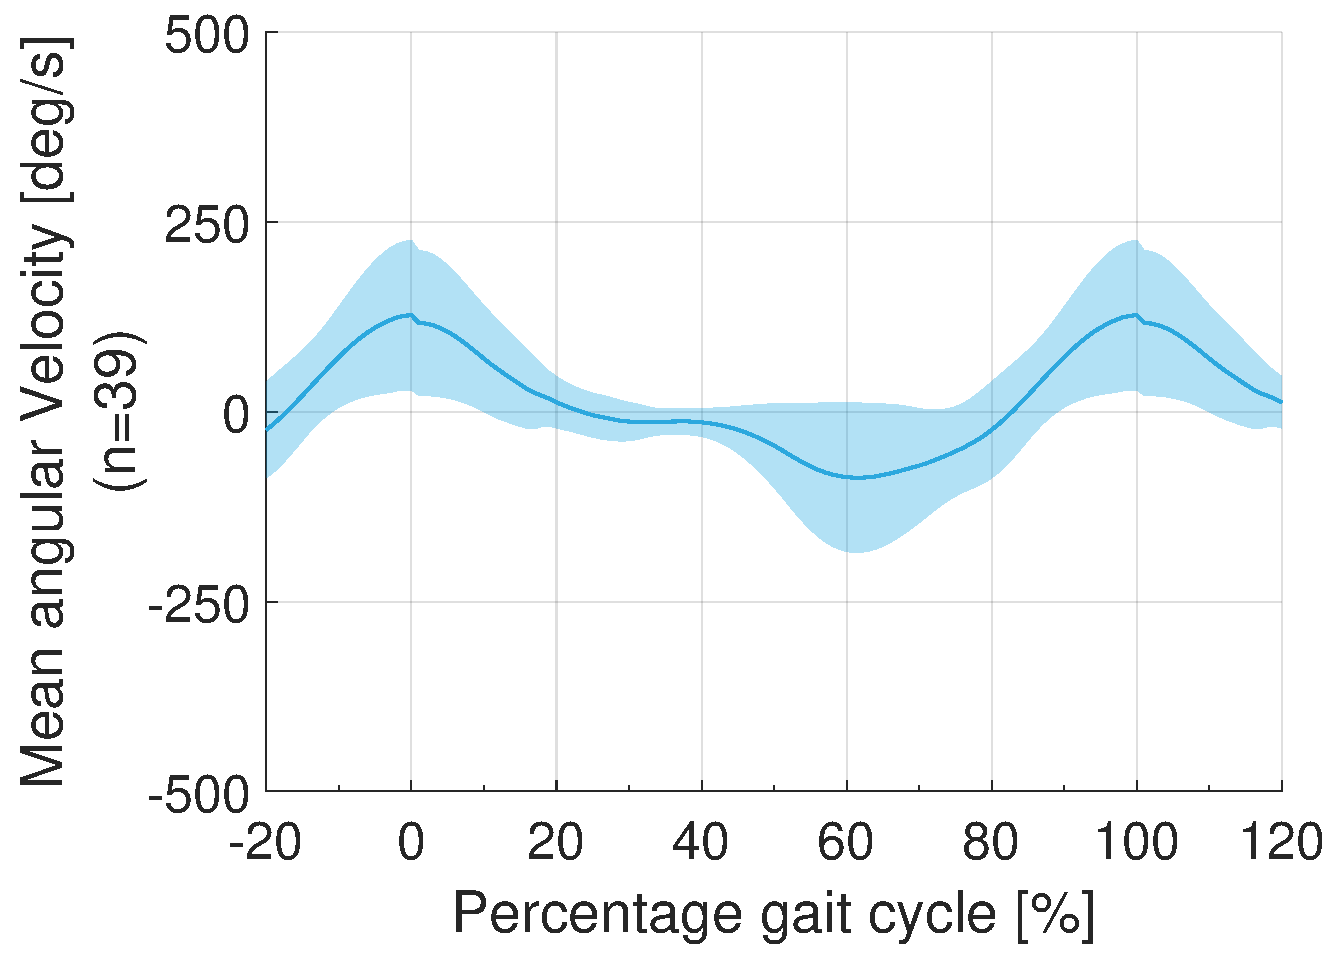
\includegraphics[width=0.275\linewidth]{content/6-Amputee/Gait-Trends/ch6_amputee_gait_trends_l_ankle_gyro_z_activity_stair_up.pdf}   &
        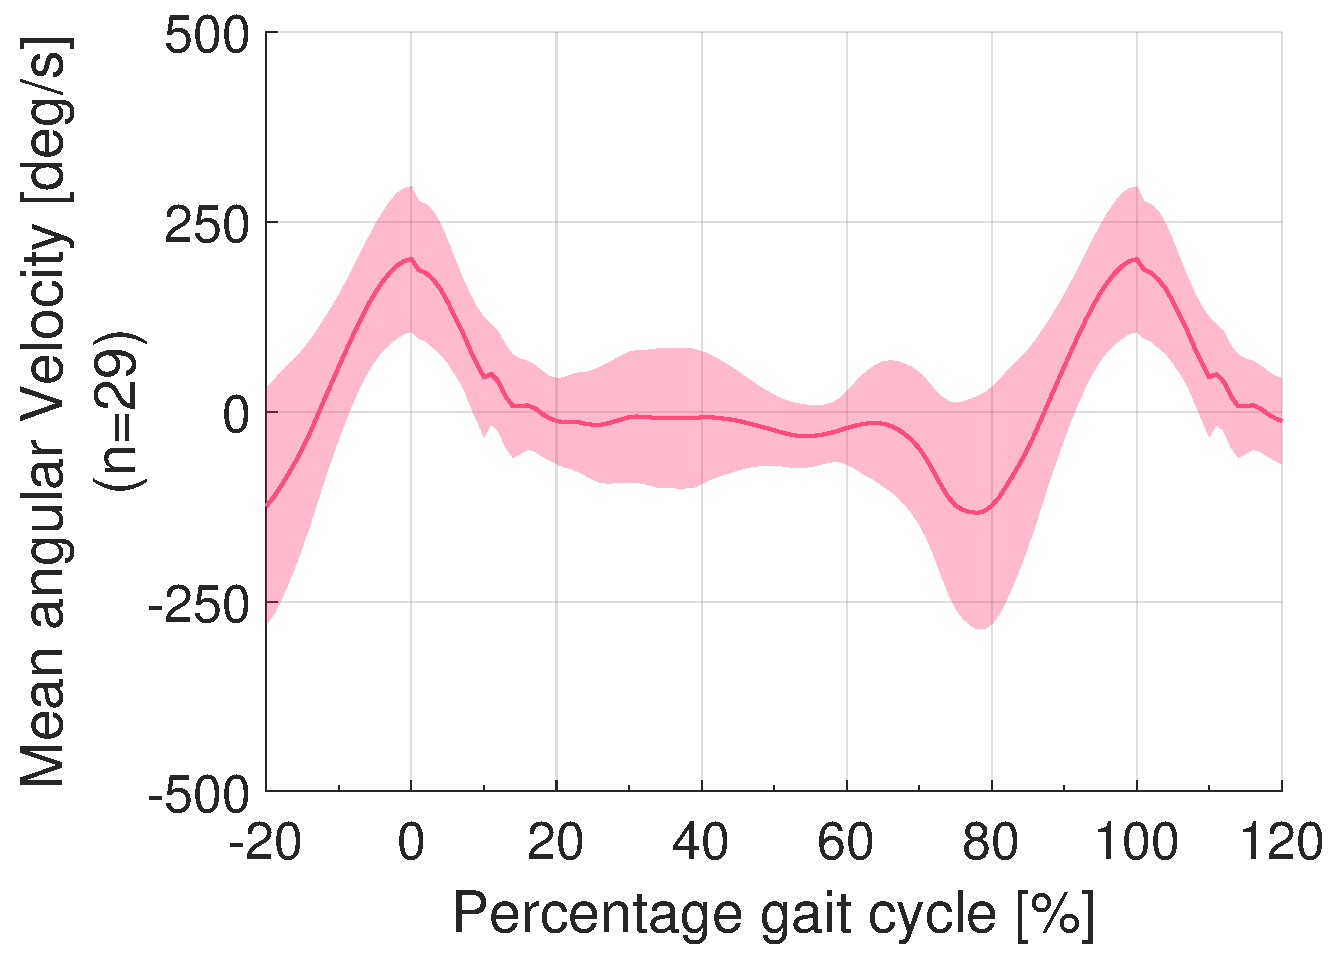
\includegraphics[width=0.275\linewidth]{content/6-Amputee/Gait-Trends/ch6_amputee_gait_trends_r_ankle_gyro_z_activity_stair_up.pdf}                                                                                                                                                                                                                                \\

        \rotatebox{90}{\quad \textbf{Stair Descent}}                                                                                             &
        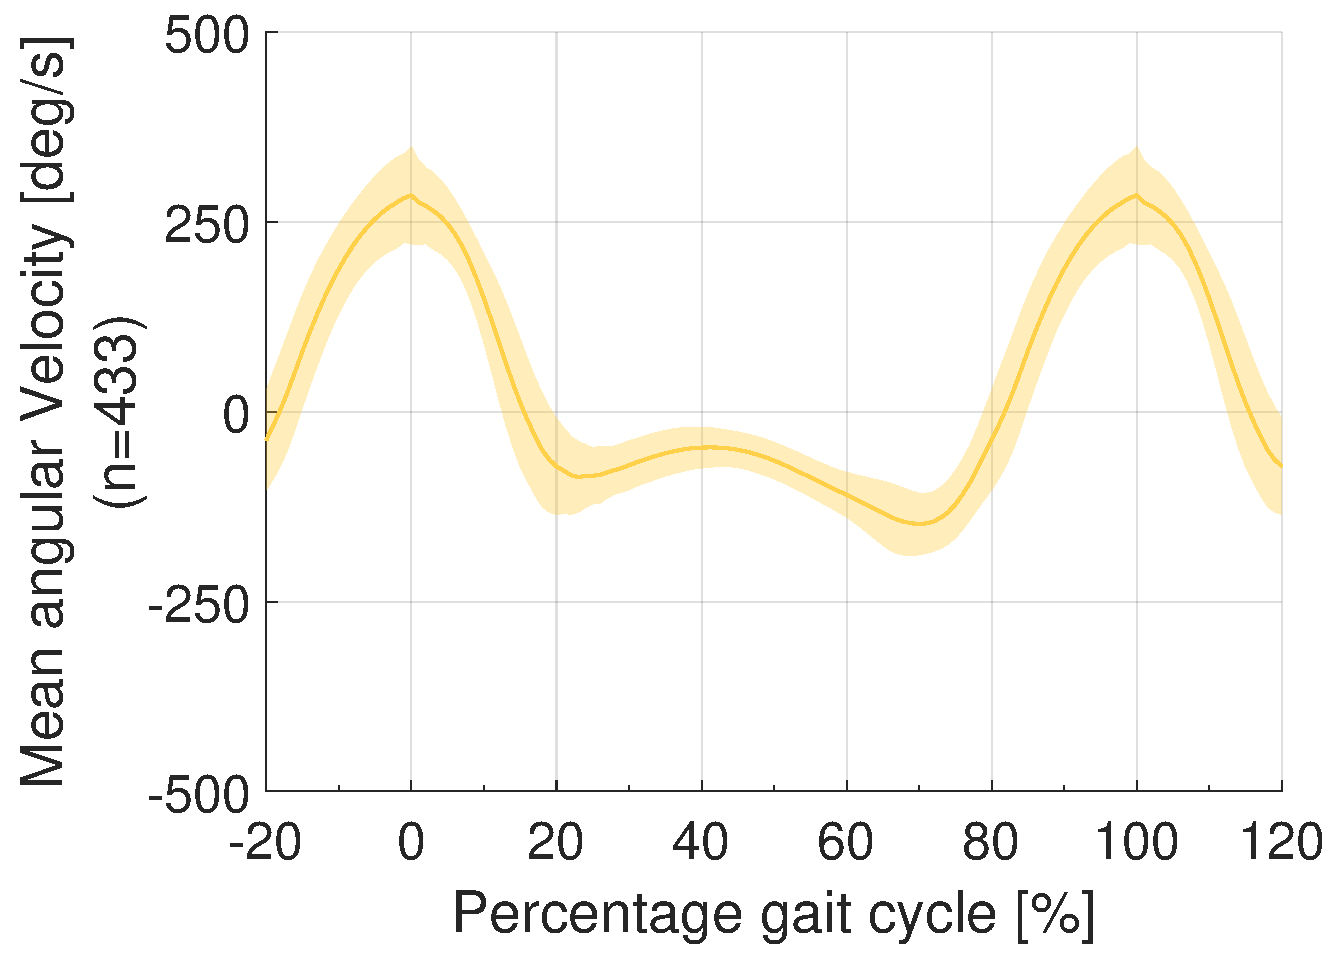
\includegraphics[width=0.275\linewidth]{content/6-Amputee/Gait-Trends/ch6_subject_01_gait_trends_r_ankle_gyro_z_activity_stair_down.pdf} & 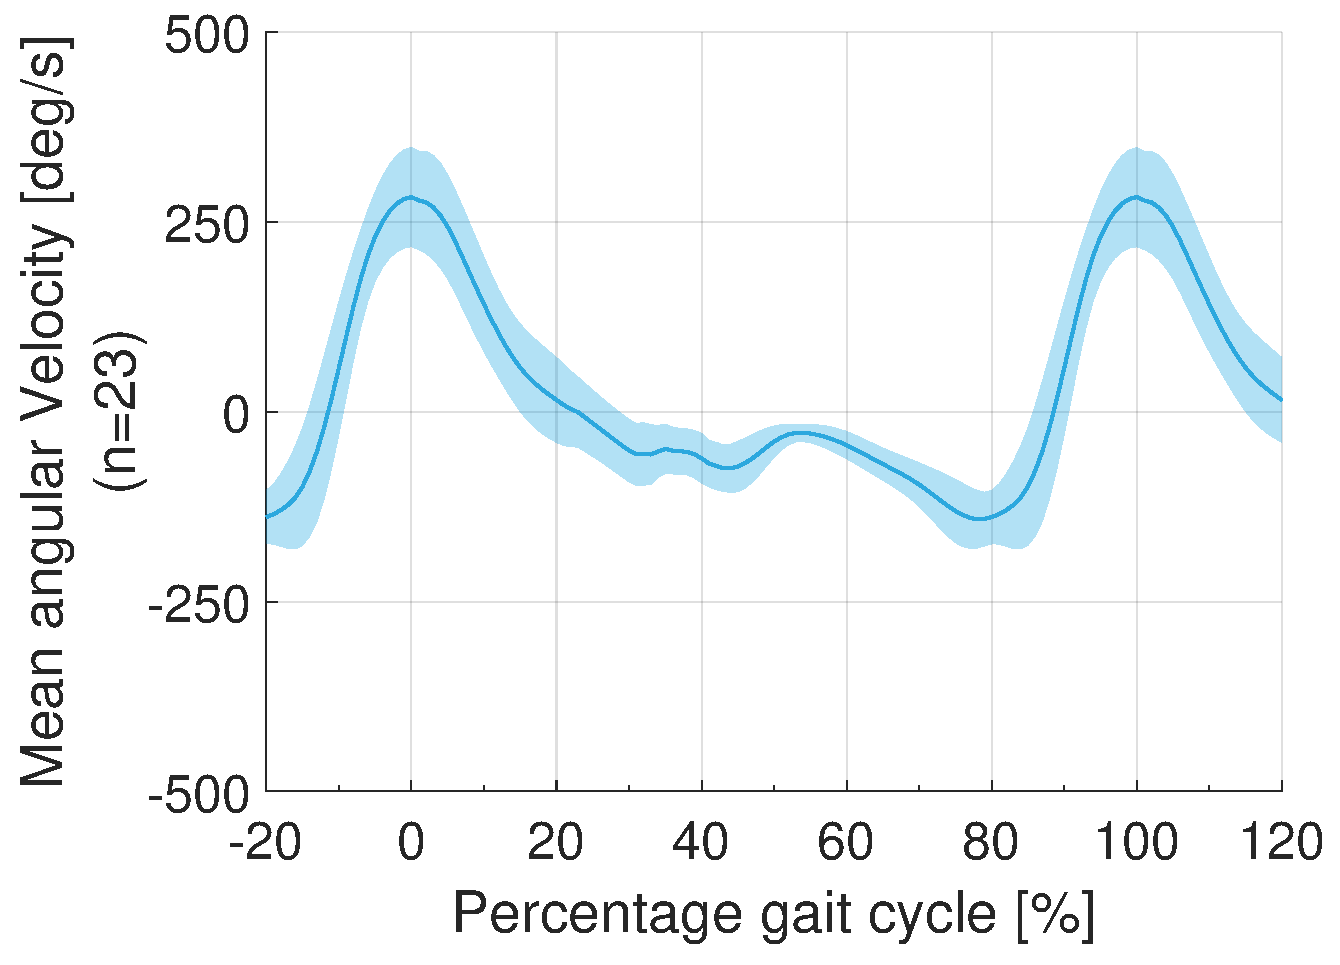
\includegraphics[width=0.275\linewidth]{content/6-Amputee/Gait-Trends/ch6_amputee_gait_trends_l_ankle_gyro_z_activity_stair_down.pdf} &
        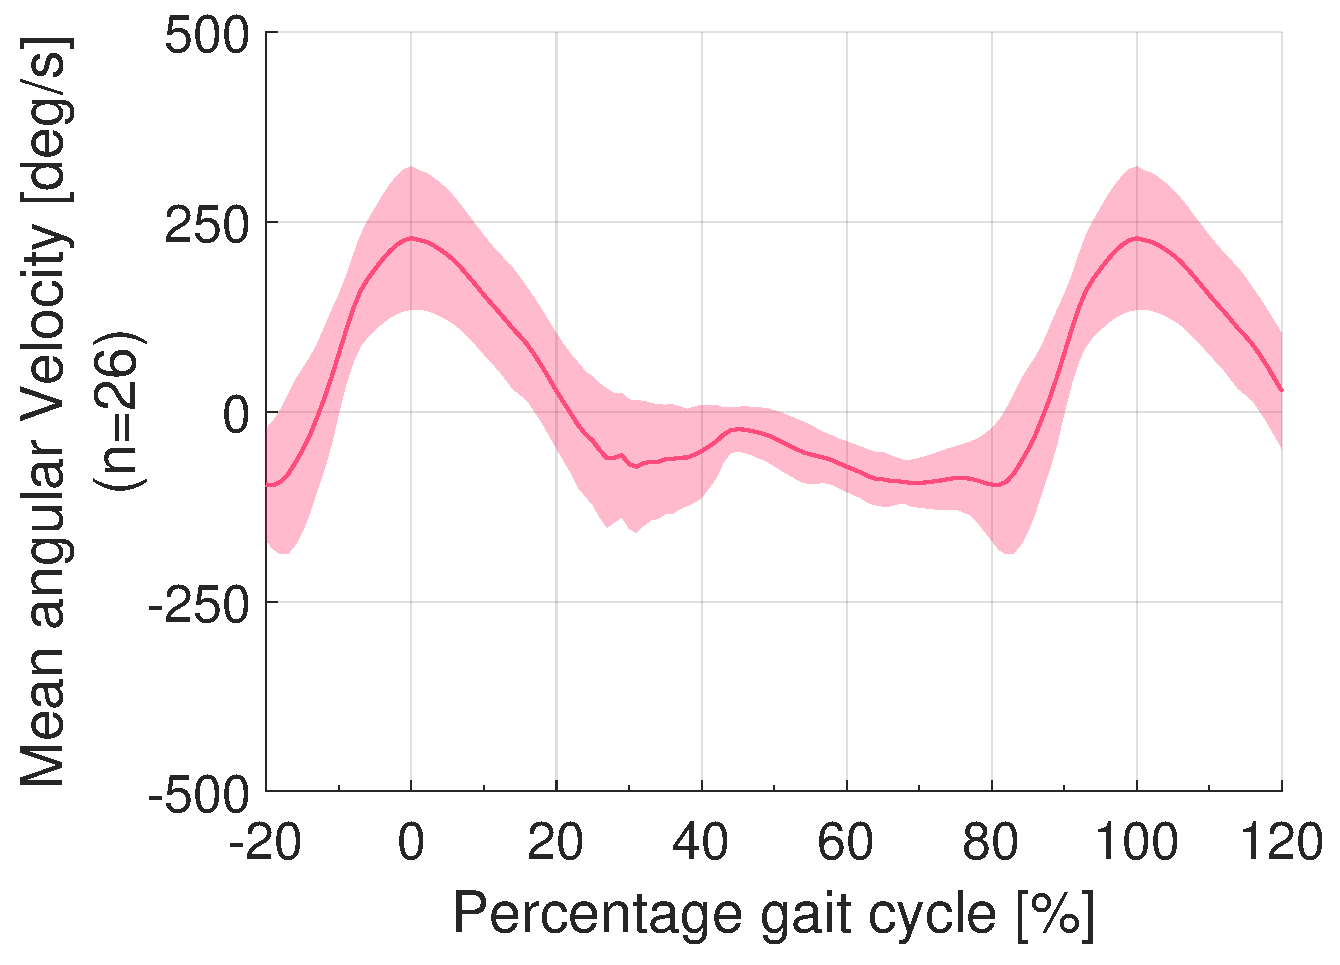
\includegraphics[width=0.275\linewidth]{content/6-Amputee/Gait-Trends/ch6_amputee_gait_trends_r_ankle_gyro_z_activity_stair_down.pdf}                                                                                                                                                                                                                              \\
    \end{tabular}
    \centering
    % \hspace*{1cm}
\includegraphics[width=0.7\textwidth]{content/6-Amputee/Gait-Trends/Legend.pdf}
    \caption[Amputee and non-amputee shank angular velocity for different activities]{Angular velocity of the shank during different activities for an amputee and non-amputee. Data is for the sagittal Plane. The yellow line is for Non-Amputee (Subject 01 Left Ankle); The red line is the intact limb of the trans-tibial amputee; The blue line is the prosthetic of the trans-tibial amputee. The solid line shows the mean of the steps recorded for each activity. The filled area represents the standard deviation.}
    \label{fig:ch6_amputee_gyro_trends}
\end{figure}

From a visual assessment of the plots, differences between the non-amputee, intact and amputated limbs can be seen. The prosthetic limb shows significant differences to both the intact and non-amputee. The non-amputee and intact limb are closer in appearance.

Differences in the prosthetic limb are especially prevalent during heel strikes (at approximately 20\% of the gait cycle), where a much lower angular velocity is observed. In general, a more significant standard deviation is also seen for the prosthetic limb, suggesting more variation in the gait between steps.

This analysis covers one axis of the gyroscope. The visible differences can also be seen in the other two gyroscope axes and accelerometer signals. As the intact limb is closer to the non-amputee, it should be expected that it will perform more highly than the prosthetic side.

%-----------------------------------------------------------------
\section{Baseline Model Performance}
\label{sec:amputee-baseline}
As before, a set of baselines are needed to determine if the personalisation methods result in a performance improvement. All baselines will be evaluated using the amputee test data sets. The two baselines will be the performance of the general models and the performance of models constructed from only the target amputee's data.

The general models were constructed in the previous Chapter from the large source data set of gait data, excluding subjects 1, 3 and 9. These are all 32 unit \acrshort{lstm} models. Both the trans-tibial amputee's right intact limb and left prosthetic limb were tested separately. The general models achieved a classification performance of $74.2\%\pm9.4$ for the intact limb. For the amputated limb, the performance was significantly lower at $55.3\%\pm9.6$. From the previous study non-amputee subjects achieved around $72\%$, this is comparably to the performance of the intact limb.

Table \ref{tab:ch6-general-model-confusion-matrix} shows the confusion matrix for the general model. The matrix shows that the general mode performs poorly on walking and stair descent for both limbs. The performance for stair descent of the prosthetic limb is notable poor.

\begin{table}[!hbt]
    \centering
    \caption[Confusion matrix of general models presented with target subject test data]{Confusion matrix of general models presented with target subject test data. Columns represent the prediction labels, and the rows represent the actual labels. Each value represents the percentage of total predicted labels for that class. (\acrfull{ra}, \acrfull{rd}, \acrfull{sa}, \acrfull{sd})}
    \label{tab:ch6-general-model-confusion-matrix}
    \begin{subtable}{\textwidth}
        \caption{Prosthetic Limb}
        \begin{tabularx}{\textwidth}{ccYYYYYY}
            \noalign{\hrule height 1.5pt}
             &                    & \multicolumn{6}{c}{\textbf{Predicted Classes}}                                                                                            \\
            \hline
             &                    & WALK                                           & \glsentryshort{ra} & \glsentryshort{rd} & \glsentryshort{sa} & \glsentryshort{sd} & STOP \\
            \multirow{6}{*}{\rotatebox{90}{\textbf{True Classes}}}
             & WALK               & 46.6                                           & 12.8               & 9.0                & 1.7                & 23.1               & 5.9  \\
             & \glsentryshort{ra} & 8.5                                            & 77.7               & 0.0                & 9.8                & 13.4               & 10.6 \\
             & \glsentryshort{rd} & 26.0                                           & 6.4                & 91.0               & 0.3                & 33.7               & 2.1  \\
             & \glsentryshort{sa} & 0.0                                            & 0.4                & 0.0                & 88.1               & 0.0                & 1.0  \\
             & \glsentryshort{sd} & 14.5                                           & 2.6                & 0.0                & 0.1                & 29.3               & 18.0 \\
             & STOP               & 4.4                                            & 0.0                & 0.0                & 0.0                & 0.6                & 62.4 \\
            \noalign{\hrule height 1.5pt}
        \end{tabularx}
    \end{subtable}
    \begin{subtable}{\textwidth}
        \caption{Intact Limb}
        \begin{tabularx}{\textwidth}{ccYYYYYY}
            \noalign{\hrule height 1.5pt}
             &                    & \multicolumn{6}{c}{\textbf{Predicted Classes}}                                                                                            \\
            \hline
             &                    & WALK                                           & \glsentryshort{ra} & \glsentryshort{rd} & \glsentryshort{sa} & \glsentryshort{sd} & STOP \\
            \multirow{6}{*}{\rotatebox{90}{\textbf{True Classes}}}
             & WALK               & 69.8                                           & 0.6                & 11.6               & 0.2                & 14.9               & 0.4  \\
             & \glsentryshort{ra} & 14.3                                           & 97.5               & 0.0                & 21.7               & 7.8                & 4.4  \\
             & \glsentryshort{rd} & 8.5                                            & 0.0                & 73.4               & 0.0                & 20.7               & 0.0  \\
             & \glsentryshort{sa} & 0.0                                            & 0.0                & 0.0                & 77.7               & 0.0                & 0.0  \\
             & \glsentryshort{sd} & 0.1                                            & 1.9                & 15.0               & 0.1                & 55.5               & 0.8  \\
             & STOP               & 7.3                                            & 0.0                & 0.0                & 0.2                & 1.1                & 94.4 \\
            \noalign{\hrule height 1.5pt}
        \end{tabularx}
    \end{subtable}
\end{table}


%------------------------
The second baseline is a set of models trained using only the amputee data. Different quantities of training windows were used to provide performance metrics for various data amounts. Figure \ref{fig:ch6-amputee-baseline-bespoke-model} shows the classification performance for both legs when tested with the test data sets. The full results of this experiment can be found in  Appendix \ref{chp:tables-of-results} Table \ref{tab:amputee-bespoke-model-table-of-results}.  The average number of epochs to train for all models was 7, with a 95\textsuperscript{th} percentile of 9.

Figure \ref{fig:ch6-amputee-baseline-bespoke-model} shows performance improving rapidly with increasing training windows levelling out after 500 samples. In all cases the prosthetic limb performs worse than the intact limb. With increasing windows the performance gap stays consistent.

Table \ref{tab:ch6-bespoke-model-confusion-matrix} shows the confusion matrix for both limbs when a bespoke model was trained with 750 training windows. This is markedly better than the confusion matrix for the general model. This backs up the observations found in the literature that general models from non-amputees perform poorly for amputees\cite{Lonini2016, Jamieson2021}. However, several classes across both limbs perform worse than the general model, suggesting the general model contains knowledge that could be used to improve performance.

\begin{table}[!hbt]
    \centering
    \caption[confusion matrix for a bespoke amputee \acrshort{lmr} model presented test data]{confusion matrix for a bespoke amputee \acrshort{lmr} model presented with test data. The 32 unit \acrshort{lstm} model was trained with 750 target data window. Columns represent the prediction labels and the rows represent the real labels. Each value represent the percentage of total predicted labels for that class. (\acrfull{ra}, \acrfull{rd}, \acrfull{sa}, \acrfull{sd})}
    \label{tab:ch6-bespoke-model-confusion-matrix}
    \begin{subtable}{\textwidth}
        \caption{Prosthetic Limb}
        \begin{tabularx}{\textwidth}{ccYYYYYY}
            \noalign{\hrule height 1.5pt}
             &                    & \multicolumn{6}{c}{\textbf{Predicted Classes}}                                                                                             \\
            \hline
             &                    & WALK                                           & \glsentryshort{ra} & \glsentryshort{rd} & \glsentryshort{sa} & \glsentryshort{sd} & STOP  \\
            \multirow{6}{*}{\rotatebox{90}{\textbf{True Classes}}}
             & WALK               & 68.2                                           & 0.6                & 42.6               & 0.6                & 0.0                & 0.0   \\
             & \glsentryshort{ra} & 9.7                                            & 94.0               & 3.8                & 1.4                & 0.5                & 0.0   \\
             & \glsentryshort{rd} & 18.9                                           & 0.4                & 53.6               & 0.2                & 0.0                & 0.0   \\
             & \glsentryshort{sa} & 0.0                                            & 0.0                & 0.0                & 79.4               & 0.0                & 0.0   \\
             & \glsentryshort{sd} & 0.0                                            & 0.0                & 0.0                & 0.0                & 99.5               & 0.0   \\
             & STOP               & 3.2                                            & 4.9                & 0.0                & 18.4               & 0.0                & 100.0 \\
            \noalign{\hrule height 1.5pt}
        \end{tabularx}
    \end{subtable}
    % \end{table}
    % \begin{table}[t]\ContinuedFloat
    %  \caption[]{confusion matrix for a bespoke amputee \acrshort{lmr} model presented with test data. The 32 unit \acrshort{lstm} model was trained with 750 target data window (Cont.).}
    \begin{subtable}{\textwidth}
        \caption{Intact Limb}
        \begin{tabularx}{\textwidth}{ccYYYYYY}
            \noalign{\hrule height 1.5pt}
             &                    & \multicolumn{6}{c}{\textbf{Predicted Classes}}                                                                                            \\
            \hline
             &                    & WALK                                           & \glsentryshort{ra} & \glsentryshort{rd} & \glsentryshort{sa} & \glsentryshort{sd} & STOP \\
            \multirow{6}{*}{\rotatebox{90}{\textbf{True Classes}}}
             & WALK               & 83.1                                           & 2.6                & 19.3               & 0.0                & 0.0                & 0.0  \\
             & \glsentryshort{ra} & 12.3                                           & 93.3               & 7.4                & 12.0               & 0.0                & 0.8  \\
             & \glsentryshort{rd} & 3.7                                            & 0.0                & 72.0               & 0.1                & 3.3                & 0.0  \\
             & \glsentryshort{sa} & 0.0                                            & 0.0                & 0.0                & 83.6               & 0.0                & 0.0  \\
             & \glsentryshort{sd} & 0.0                                            & 0.0                & 0.0                & 0.0                & 96.7               & 0.0  \\
             & STOP               & 0.9                                            & 4.1                & 1.2                & 4.3                & 0.0                & 99.2 \\
            \noalign{\hrule height 1.5pt}
        \end{tabularx}
    \end{subtable}
\end{table}

\begin{figure}[H]
    \centering
    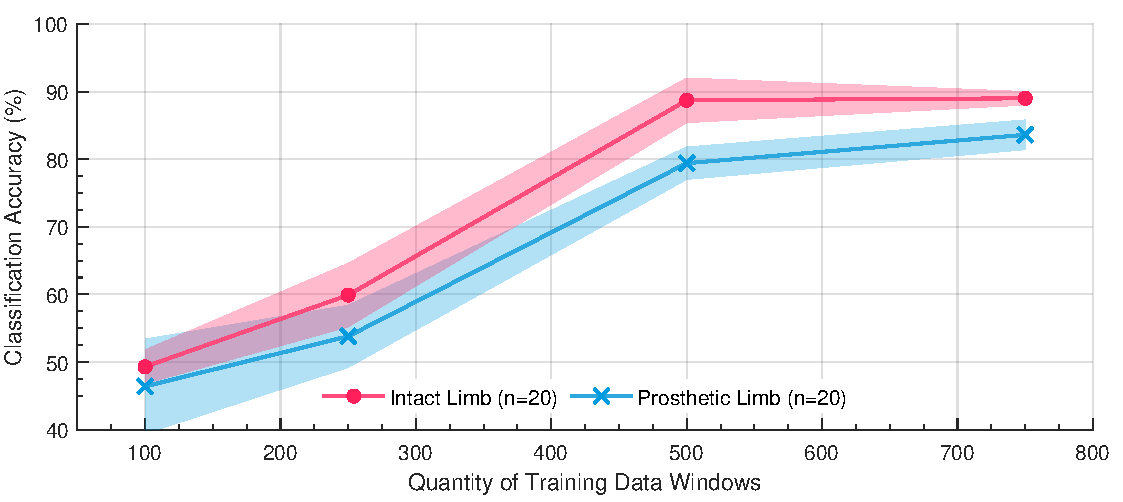
\includegraphics[width=\textwidth]{content/6-Amputee/ch6_baseline_model_accuracy.pdf}
    \caption[Classification accuracy using increasing quantities of amputee target data]{Classification accuracy for HAR model using increasing quantities of only amputee target data. The red line shows the performance of the trained model on the intact limb of a trans-tibial amputee. The blue line shows the performance of the trained model for the prosthetic side. The filled areas represent the standard deviation (n=20).}
    \label{fig:ch6-amputee-baseline-bespoke-model}
\end{figure}


%-----------------------------------------------------------------
\section{Data supplementation} % Are we going to include this?
\label{sec:amputee-supplementation}
The first personalised model technique that will be investigated is data supplementation. This involves supplementing target data with a varying amount of data from a general source set to form a large training set. The source data is made up of a larger number of non-amputee subjects.

The experiment consisted of mixing 100, 250, 500 and 750 target data windows with between 100 and 3000 source windows. On average, each model took 10 epochs to train, 95\textsuperscript{th} percentile of 17. In general, the more data used, the larger the number of epochs required. Table \ref{tab:ch6-classfication-accuracy-mixed-source-target-right} shows classification performance for all combinations.

As before, the performance of the prosthetic side is lower than the intact side. All classification accuracies for the prosthetic exceed the general model performance. However, the lowest two results for 100 source windows perform worse than the general model for the intact limb.

For the intact side, none of the 500 and 750 target window models exceeds the performance of the bespoke models with the same quantity of target windows. For the amputated side, all but 750 target window, 100 source window result exceed the bespoke model performance.

At a lower value of target windows, a higher quantity of source windows improves performance; less source data is needed at higher target windows. At higher values of target data windows, the performance improvement is minimal, especially for the intact side. This suggests that this method may become less valuable the more target data available.

\begin{table}[!hbt]
    \caption[Table of classification accuracy for amputee test data for a model trained using varying amounts of Source and Target training data]{Table of classification accuracy for amputee test data for a model trained using varying amounts of Source and Target training data. The cell value represents the percentage classification accuracy $\pm\sigma$ $(n=8)$. The highest classification accuracy for each quantity of target windows has been highlighted in bold}
    \label{tab:ch6-classfication-accuracy-mixed-source-target-right}
    \centering
    \begin{subtable}{\textwidth}
        \centering
        \caption{Intact Limb} % Right
        \begin{tabularx}{0.99\textwidth}{cr| *{4}{Y}}
            \noalign{\hrule height 1.5pt}
             &      & \multicolumn{4}{c}{\textbf{Target Training Windows}}                                                                                                                                           \\
             &      & 100                                                  & 250                                         & 500                                         & 750                                         \\
            \hline
            \multirow{7}{*}{\rotatebox{90}{\parbox{3.4cm}{\centering\textbf{Source Training                                                                                                                          \\Windows}}}}
             & 0    & $0.428{\scriptscriptstyle\pm0.05}$                   & $0.448{\scriptscriptstyle\pm0.05}$          & $0.863{\scriptscriptstyle\pm0.02}$          & $0.869{\scriptscriptstyle\pm0.01}$          \\
             & 100  & $0.717{\scriptscriptstyle\pm0.03}$                   & $0.682{\scriptscriptstyle\pm0.02}$          & $0.879{\scriptscriptstyle\pm0.02}$          & $0.877{\scriptscriptstyle\pm0.04}$          \\
             & 250  & $0.764{\scriptscriptstyle\pm0.04}$                   & $0.730{\scriptscriptstyle\pm0.03}$          & $0.883{\scriptscriptstyle\pm0.03}$          & $\mathbf{0.889{\scriptscriptstyle\pm0.01}}$ \\
             & 500  & $0.800{\scriptscriptstyle\pm0.04}$                   & $0.795{\scriptscriptstyle\pm0.03}$          & $0.875{\scriptscriptstyle\pm0.02}$          & $0.888{\scriptscriptstyle\pm0.02}$          \\
             & 750  & $0.815{\scriptscriptstyle\pm0.01}$                   & $0.801{\scriptscriptstyle\pm0.02}$          & $0.873{\scriptscriptstyle\pm0.02}$          & $0.881{\scriptscriptstyle\pm0.02}$          \\
             & 1000 & $0.801{\scriptscriptstyle\pm0.04}$                   & $0.786{\scriptscriptstyle\pm0.03}$          & $\mathbf{0.886{\scriptscriptstyle\pm0.03}}$ & $0.874{\scriptscriptstyle\pm0.02}$          \\
             & 1500 & $\mathbf{0.835{\scriptscriptstyle\pm0.03}}$          & $0.794{\scriptscriptstyle\pm0.06}$          & $0.871{\scriptscriptstyle\pm0.01}$          & $0.875{\scriptscriptstyle\pm0.03}$          \\
             & 3000 & $0.825{\scriptscriptstyle\pm0.01}$                   & $\mathbf{0.826{\scriptscriptstyle\pm0.07}}$ & $0.846{\scriptscriptstyle\pm0.03}$          & $0.863{\scriptscriptstyle\pm0.03}$          \\
            \noalign{\hrule height 1.5pt}                                                                                                                                                                            \\
        \end{tabularx}
    \end{subtable}

    \begin{subtable}{\textwidth}
        \centering
        \caption{Prosthetic Limb} % Left
        \begin{tabularx}{0.99\textwidth}{cr| *{4}{Y}}
            \noalign{\hrule height 1.5pt}
             &      & \multicolumn{4}{c}{\textbf{Target Training Windows}}                                                                                                                                           \\
             &      & 100                                                  & 250                                         & 500                                         & 750                                         \\
            \hline
            \multirow{7}{*}{\rotatebox{90}{\parbox{3.4cm}{\centering\textbf{Source Training                                                                                                                          \\Windows}}}}
             & 0    & $0.447{\scriptscriptstyle\pm0.02}$                   & $0.469{\scriptscriptstyle\pm0.03}$          & $0.765{\scriptscriptstyle\pm0.04}$          & $0.830{\scriptscriptstyle\pm0.03}$          \\
             & 100  & $0.626{\scriptscriptstyle\pm0.05}$                   & $0.643{\scriptscriptstyle\pm0.03}$          & $0.855{\scriptscriptstyle\pm0.02}$          & $0.813{\scriptscriptstyle\pm0.04}$          \\
             & 250  & $0.714{\scriptscriptstyle\pm0.04}$                   & $0.611{\scriptscriptstyle\pm0.02}$          & $0.836{\scriptscriptstyle\pm0.05}$          & $0.843{\scriptscriptstyle\pm0.03}$          \\
             & 500  & $0.752{\scriptscriptstyle\pm0.03}$                   & $0.729{\scriptscriptstyle\pm0.08}$          & $0.842{\scriptscriptstyle\pm0.02}$          & $0.840{\scriptscriptstyle\pm0.05}$          \\
             & 750  & $0.734{\scriptscriptstyle\pm0.06}$                   & $0.712{\scriptscriptstyle\pm0.04}$          & $0.848{\scriptscriptstyle\pm0.03}$          & $0.847{\scriptscriptstyle\pm0.02}$          \\
             & 1000 & $0.756{\scriptscriptstyle\pm0.02}$                   & $0.756{\scriptscriptstyle\pm0.08}$          & $\mathbf{0.875{\scriptscriptstyle\pm0.03}}$ & $\mathbf{0.872{\scriptscriptstyle\pm0.01}}$ \\
             & 1500 & $0.734{\scriptscriptstyle\pm0.02}$                   & $\mathbf{0.764{\scriptscriptstyle\pm0.05}}$ & $0.869{\scriptscriptstyle\pm0.02}$          & $0.852{\scriptscriptstyle\pm0.02}$          \\
             & 3000 & $\mathbf{0.767{\scriptscriptstyle\pm0.02}}$          & $\mathbf{0.764{\scriptscriptstyle\pm0.04}}$ & $0.874{\scriptscriptstyle\pm0.02}$          & $0.849{\scriptscriptstyle\pm0.02}$          \\
            \noalign{\hrule height 1.5pt}                                                                                                                                                                            \\
        \end{tabularx}
    \end{subtable}
\end{table}



%-----------------------------------------------------------------
\section{Transfer Learning}
\label{sec:amputee-transfer}
Transfer learning involves using the knowledge captured in an existing model as a starting point to building a personalised model. For this experiment, five general models constructed in Chapter \ref{chp:personalisation} were used as the starting point. Varying quantities of target amputee data windows were then used to fine-tune these starting models to personalise them to the amputee. By freezing the different network layers, attempts to reduce the computation load required to train the model could be made.

Figure \ref{fig:ch6-amputee-retrain-pre-trained} shows three different experiments in transfer learning. Each trained different layers of the network. The first trained all layers, the second just the dense layer, and finally just the \acrshort{lstm} layer.

\begin{figure}[!hbtp]
    \centering
    \begin{subfigure}{\textwidth}
        \centering
        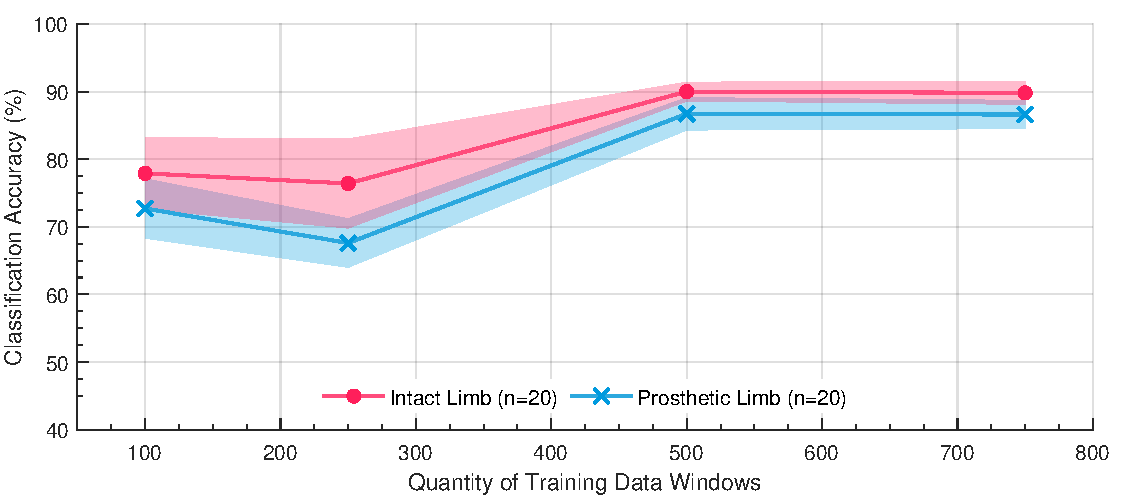
\includegraphics[width=\textwidth]{content/6-Amputee/ch6_pre_trained_model_accuracy.pdf}
        \caption{Fine tuning all layers}
    \end{subfigure}
    \begin{subfigure}{\textwidth}
        \centering
        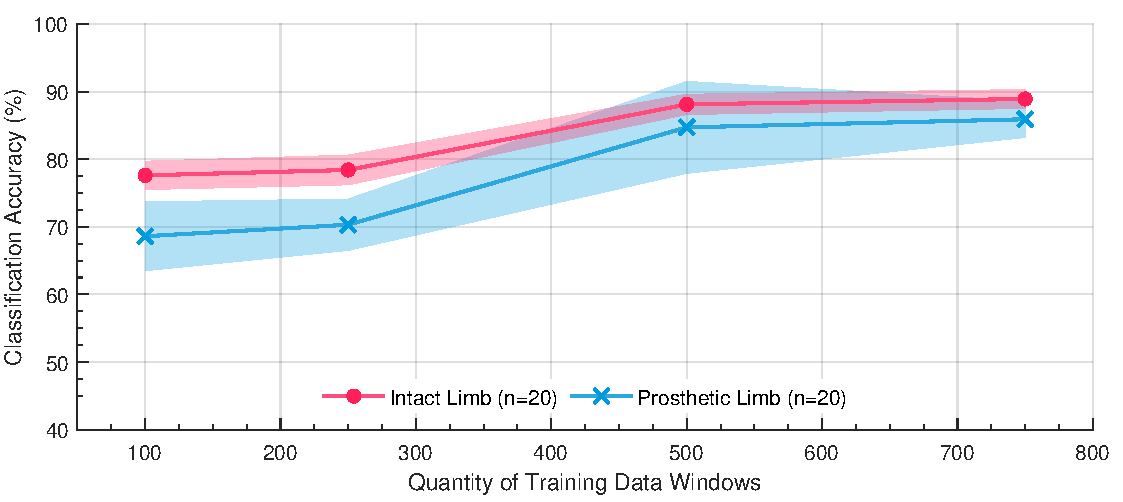
\includegraphics[width=\textwidth]{content/6-Amputee/ch6_frozen_lstm_layer_accuracy.pdf}
        \caption{Fine tuning only the dense layer}
    \end{subfigure}
    \caption[Accuracy of re-training a pre-trained model using amputee target data]{Classification accuracy for re-training a pre-trained model using increasing quantities of amputee target data. The red line shows the performance of the trained model on the intact limb of a trans-tibial amputee. The blue line shows the performance of the trained model for the prosthetic side. The filled areas represent the standard deviation (n=20).}
    \label{fig:ch6-amputee-retrain-pre-trained}
\end{figure}
\begin{figure}[t]\ContinuedFloat
    \centering
    \begin{subfigure}{\textwidth}
        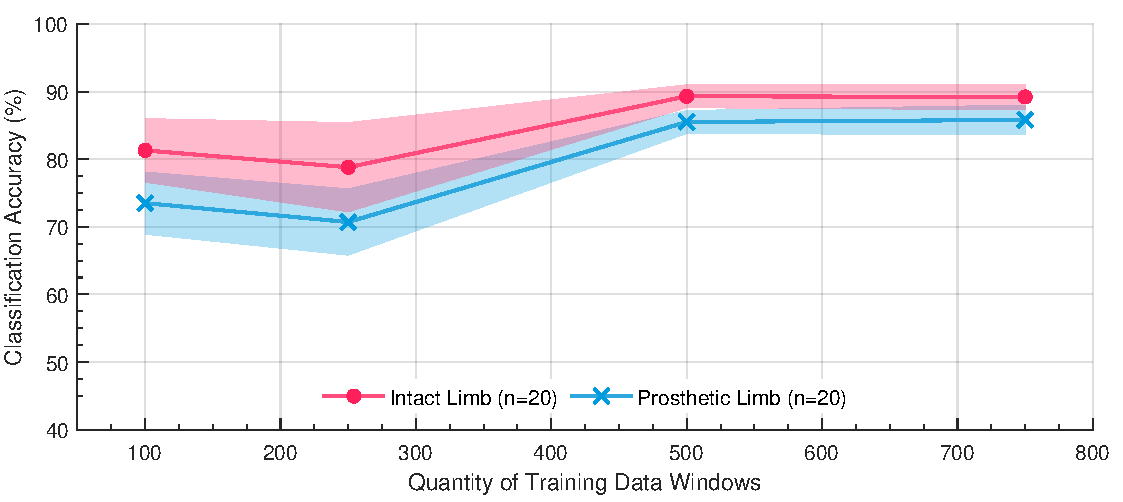
\includegraphics[width=\textwidth]{content/6-Amputee/ch6_frozen_dense_layer_accuracy.pdf}
        \caption{Fine tuning only the \acrshort{lstm} layer}
    \end{subfigure}
    \caption[]{Classification accuracy for re-training a pre-trained model using increasing quantities of amputee target data (Cont.).}
\end{figure}

On average, each model took 6 epochs 95\textsuperscript{th} percentile of 10. In general, the more data used, the larger the number of epochs required.

When training all layers, classification performance significantly increased over the base general model with only a few target windows. For the prosthetic side with 100 target windows, there was a $22\%$ increase in performance over the general model. This reduced to just under $1\%$ for the intact limb at 750 windows. The improvement over the bespoke model slightly higher achieving at least a $3\%$ improvement. Overall transfer learning resulted in an improvement for all configurations.

Fine-tuning only the dense layer did not result in better performance than fine-tuning all layers and for the intact limb at 500 and 750 windows was worse than the baseline bespoke model. Using this method significantly increased standard deviation for the prosthetic limb, although slightly reduced $\sigma$ for the intact limb.

Fine-tuning only the \acrshort{lstm} layer gave the best performance for 100 and 250 target windows compared to fine-tuning all layers. Performance was a couple of percent better; however, the higher two target window quantities performance was approximately a percent worse. The standard deviation remained roughly the same. On balance, it showed no improvement over fine-tuning all layers.

%-----------------------------------------------------------------
\section{Discussion and Conclusions}
\label{sec:amputee-discussion}
The work in this Chapter set out to investigate if the personalisation methods for an \acrshort{lmr} classifier developed in Chapter \ref{chp:personalisation} were applicable to an amputee. A set of comparable data was collected from a trans-tibial amputee to achieve this. This was then used to repeat the previous experiments for the amputee subject.

Jamieson and Lonini suggested that the direct use of a general model trained using only non-amputee data would not perform adequately for a person with gait impairments\cite{Lonini2016, Jamieson2021}. This was borne out in the results when data from the prosthetic limb was tested. It achieved a classification accuracy of $55.3\%$, significantly less than the non-amputee subjects.

When data from the amputee's intact limb was used, classification performance was much higher. The test subject has a significant asymmetry in their gait, with the intact side matching more closely to the source non-amputees gait. This is an area that requires additional research as it is potentially an easy way to improve the performance of an amputee gait classifier.

Both the data supplementation and transfer learning approaches improved over the baseline classifiers. The differences observed in the previous Chapter were again shown. The quantity of source data required for data supplementation was hard to predict, and only training specific layers for transfer learning resulted in minimal changes. As before, the transfer learning performance appeared to perform more consistently and required significantly less computing resources to train.

The overall performance of both the bespoke model and personalised models at 500 and 750 training windows was significantly higher than seen in the previous Chapter. They also looked more likely to be levelling off in performance. There are two likely reasons for this. First, a much smaller testing set was used, so the trained model was tested with a narrower range of environments. Secondly, all the amputee data was collected at a single site, and therefore the training data is likely to include environments seen in the test set. The division of stairs episodes would also have a similar effect.

Further, as data for only one amputee was collected, it is not possible to say whether these methods are more generally applicable. To test the results further, more amputees and more data per amputee are required.

In the previous Chapter, a method for improving data supplementation was data grouping. It is unlikely to be successful in this scenario due to the likely difficulty in finding subjects with a similar gait to an amputee. However, there may be potential in including more persons with gait impairments to improve the networks ability to adapt. This is a potential area for further research.

No literature was found investigating the classification performance difference between the two lower limbs of an amputee or other person with asymmetric gait. The results consistently showed that classification of the intact limb had higher accuracies than the amputated limb. This could be an exciting area of research for improving the classifier's performance using both sides of the body. A form of ensemble network could be a good candidate for this.

The personalisation approach shows promise in the area of amputee gait classification. As concluded in the previous chapter the general training population should ideally contain individuals of similar gait to the target subject. This is significantly harder for amputees. Further research is required in this area to exploit the potential for using non-amputee data to reduce data requirements for amputees and to investigate the limitations of this approach. Further research into the use of the intact limb to improve classification performance is also required,
